\documentclass[9pt,twocolumn,twoside]{rilabRxiv}
% Use the documentclass option 'lineno' to view line numbers
\setlength{\marginparwidth}{2cm}
\usepackage[textsize=tiny,colorinlistoftodos]{todonotes} % comments in margins
\definecolor{cornflowerblue}{rgb}{0.39, 0.58, 0.93}
\usepackage{multicol}


%%%%%%%Add comments in color
\newcommand{\ms}[1]{{\small \textcolor{green}{#1}}}
\newcommand{\jri}[1]{{\small \textcolor{red}{#1}}}
\newcommand{\citex}[1]{{\small \textcolor{red}{CITE(#1)}}}
\newcommand{\X}{{\textcolor{red}{X}}}

\newcolumntype{b}{X}
\newcolumntype{s}{>{\hsize=.5\hsize}X}

% Set supplement numbers to S and start counting newly
\newcommand{\beginsupplement}{%
        \setcounter{table}{0}
        \renewcommand{\thetable}{S\arabic{table}}%
        \setcounter{figure}{0}
        \renewcommand{\thefigure}{S\arabic{figure}}%
     }


\usepackage{hyperref}

\title{Timing is key in determining the impacts of demography on linked selection}

\author[$\dagger$,]{Raul Torres}
\author[$\ast$]{Markus Stetter}
\author[$\dagger$,1]{Ryan Hernandez}
\author[$\ast$,$\ddagger$,1]{Jeffrey Ross-Ibarra}

\affil[$\dagger$]{Some other Department, Some other place, CA, USA}
\affil[$\ast$]{Dept. of Plant Sciences and Center for Population Biology, University of California, Davis, CA, USA}
\affil[$\dagger$]{Some other Department, Some other place, CA, USA}
\affil[$\ddagger$]{Genome Center, University of California, Davis, CA, USA}


\keywords{Keyword one, keyword 2}

\runningtitle{Demography and background selection} % For use in the footer

%% For the footnote.
%% Give the last name of the first author if only one author;
% \runningauthor{FirstAuthorLastname}
%% last names of both authors if there are two authors;
% \runningauthor{FirstAuthorLastname and SecondAuthorLastname}
%% last name of the first author followed by et al, if more than two authors.
\runningauthor{Torres, Stetter \textit{et al.}}


%%% Abstract %%%%%%%%%%%%%%%%%%
\begin{abstract}
Neutral genetic diversity across the genome is determined by the complex interplay of mutation, demographic history, and natural selection. While the direct action of natural selection is limited to functional loci across the genome, its impact can have effects on nearby neutral loci due to genetic linkage. These effects of selection at linked sites, referred to as genetic hitchhiking and background selection (BGS), are pervasive across natural populations. However, only recently has there been a focus on the joint consequences of demography and selection at linked sites, and empirical studies have sometimes come to apparently contradictory conclusions. In order to understand the relationship between demography and linked selection, we conducted an extensive forward simulation study of BGS under a range of demographic models. We found that levels of diversity compared to an equilibrium population vary  over time, and that the initial dynamics after a population size change are often in the opposite direction of the long-term expected trajectory. Our detailed observations of the temporal dynamics of neutral diversity in the context of selection at linked sites in nonequilibrium populations provides new intuition about why patterns of diversity under BGS vary through time in natural populations and helps reconcile previously contradictory observations.
Most notably, our results highlight that classical models of BGS are poorly suited for predicting diversity in nonequilibrium populations.
\end{abstract}
%%%%%%%%%%%%%%%%%%%%%%%%%%

\setboolean{displaycopyright}{false}

\begin{document}
\begin{multicols}{1}
\maketitle
\end{multicols}
\thispagestyle{firststyle}
%\firstpagefootnote
\correspondingauthoraffiliation{
Dept. of Plant Sciences, University of California, Davis, CA, USA
E-mail: rossibarra@ucdavis.edu \\
Genome Quebec Innovation Center, McGill University, Montreal, Canada
E-mail: ryan@McGill.edu}
\vspace{-11pt}%


\section{Introduction}
\lettrine[lines=2]{\color{color2}T}{}
he effects of natural selection and demography on neutral genetic diversity within populations have long been of interest in evolutionary and population genetics.
Recent efforts in sequencing tens of thousands of genomes across a multitude of species have yielded new and valuable insights into how these two forces of evolution have shaped extant patterns of genomic variation.
Yet, while the theoretical underpinnings of the effects of natural selection and demography on genetic diversity have been investigated for decades \citep{smith1974hitch, nei1975bottleneck, maruyama1984population, maruyama1985population, kaplan1989hitchhiking, charlesworth1993effect, nordborg1996effect, hudson1995deleterious, tajima1989effect}, detailed investigation into how they jointly act to create patterns of diversity in different populations remains lacking.

Both theory and empirical observation have long shown that patterns of neutral genetic variation can vary regionally across the genome as a function of recombination rate \citep{smith1974hitch, begun1992levels}.
This is because natural selection operating on selected sites not only decreases genetic variation at the focal site but can also lead to decreases in nearby neutral genetic diversity due to genetic linkage \citep{cutter2013genomic}.
These effects, known as genetic hitchhiking \citep{smith1974hitch}[1] (in which neutral variants rise to high frequency with adaptive variants) and background selection \citep{charlesworth1993effect} (BGS; in which neutral variants are removed along with deleterious variants) can be widespread across the genome.
Evidence for selection at linked sites has been found across an array of species, including \textit{Drosophila melanogaster} \citep{begun1992levels, comeron2014background, charlesworth1996background, andolfatto2007hitchhiking, sella2009pervasive, elyashiv2016genomic}, wild and domesticated rice \citep{flowers2011natural, xu2012resequencing}, \textit{Capsella} \citep{williamson2014evidence}, maize \citep{beissinger2016recent}, and humans \citep{sabeti2002detecting, reed2005fitting, voight2006map, mcvicker2009widespread, cai2009pervasive, hernandez2011classic, lohmueller2011natural}.

Demographic change can also impact patterns of diversity across the genome.
For example, neutral theory predicts that the amount of genetic diversity is proportional to a population’s effective population size (\textit{$N_e$}), such that changes in \textit{$N_e$} should result in concomitant changes to diversity \citep{kimura1983neutral}[28].
However, evidence suggests that such diversity also varies much less in magnitude across species when compared to their census population sizes \citep{lewontin1974genetic, leffler2012revisiting}[29,30].
One of the most common forms of a population size change is a population bottleneck, whereby populations suffer a large decrease followed by an expansion.
Bottlenecks can occur via domestication events \citep{doebley2006molecular, tang2010domestication, wiener2011deciphering, gaut2018demography}[31–34], seasonal or cyclical fluctuations in population size \citep{elton1924periodic, ives1970further, itoh2009seasonal, noren2014genetic}[35–38], and founder events \citep{henn2012great, dlugosch2008founding, david1988genetic}[39–41].
Notably, while the rate of loss of diversity in response to a population contraction is quite fast, the recovery of diversity from a following population increase can be quite slow [42].
As a result,  large contemporary populations may still yield patterns of low average genetic diversity if their population size was much smaller in the recent past.
In humans, this is clearly evident in European and Asian populations due to the out-of-Africa bottleneck [43].

Because selection at linked sites and demography are both pervasive forces across a multitude of species, the characterization of how these two forces interact with one another is necessary in order to develop a full picture on the determinants of neutral genetic diversity.
The efficiency of natural selection scales proportionally with Ne and the impact of selection at linked sites on neutral diversity is likely to be greater in larger populations and lower in smaller populations [5,11,44], although the rate of change for lowered diversity may diminish as populations reach larger and larger sizes [45,46].
Further, demographic changes can also increase (in the case of bottlenecks) or decrease (in the case of expansions) the rate of drift.
It is therefore plausible that the rate at which diversity at a neutral locus is perturbed by selection at linked sites could be highly dependent on both the current as well as long-term Ne of the population.
This competition between “genetic draft” (which increases with N) and genetic drift (which decreases with N) may be a key contributor to the limited range of diversity observed among species  despite much larger observed differences in census size [44–46].
However, selection at linked sites alone may not be sufficient to explain the observed discrepancy between observed diversity and census populations sizes [47], and the action of both demography and selection at linked sites in concert may provide a better model.

Many models of selection at linked sites were also formulated with the assumption that the population is large enough (or selection strong enough) such that mutation-selection balance is maintained [6,48,49].
However, non-equilibrium demographic change may break such assumptions and forces other than selection may drive patterns of variation in regions experiencing selection at linked sites.
For example, during the course of a population bottleneck, genetic drift may transiently dominate the effects of selection at many sites such that traditional models of selection will poorly predict patterns of genetic diversity.
But linked selection may also exacerbate the impact of genetic drift, resulting in even greater losses than expected by the action of demography alone.
A recent review by \citet{comeron2017background}  included a cursory investigation into the impact of demography on diversity in regions under BGS and suggested a dependency on demographic history.
Recent empirical work in maize and humans has also demonstrated a strong interaction between demography and selection at linked sites \citep{beissinger2016recent,torres2018human}.
But these papers also demonstrate the need for a deeper understanding of the interaction between demography and selection at linked sites, as the two studies come to opposing conclusions about the impact of population bottlenecks and expansion on patterns of diversity  in regions affected by selection at linked sites.

In order to more fully explore the joint consequences of demography and selection at linked sites, in this study we conducted extensive simulations of different demographic models jointly with the effects of BGS.
We find that the time span removed from demographic events is critical for populations experiencing non-equilibrium demography and can yield contrasting patterns of diversity that reconciles apparently contradicting results  \citep{beissinger2016recent,torres2018human}.
Additionally, the sensitivity of genetic diversity to demography is dependent on the frequency of the alleles being measured, with rare variants experiencing more dynamic changes through time.

Our results demonstrate that traditional models of selection at linked sites may be poorly suited for predicting patterns of diversity for populations experiencing recent demographic change, and that the predicted forces of BGS become apparent only after populations begin to approach equilibrium.
Importantly, even simple intuition about the effect of selection at linked sites may lead to erroneous conclusions if populations are assumed to be at equilibrium.
These results should motivate further research into this area and support the use of models that incorporate the joint effects of both demography and selection at linked sites.

\section{Materials and Methods}
\label{sec:materials:methods}

\subsection{Simulation model}

We simulated a diploid and randomly mating population using fwdpy11 v1.2a (\href{https://github.com/molpopgen/fwdpy11}{\emph{https://github.com/molpopgen/fwdpy11}}), a Python package using the fwdpp library [52].
Selection parameters for simulating BGS followed those of Torres et al. 2018 [51], with deleterious variation occurring at 20\% of sites across a 2 Mb locus and the selection coefficient, \textit{s}, drawn from two distributions of fitness effects (DFE).
Specifically, 13\% of deleterious sites were drawn from a gamma distribution (parameters: mean = $\alpha/\beta$, variance = $\alpha/\beta^2$) parameterized Gamma($\alpha = 0.0415$, $\beta = 80.11$) and seven percent from a distribution parameterized Gamma($\alpha = 0.184$, $\beta = 6.25$).
These distributions mimic the DFEs inferred across non-coding and coding sites within the human genome [53,54].
Fitness followed a purely additive model in which the fitness effect of an allele was 0, $0.5s$, and $s$ for homozygous ancestral, heterozygous, and homozygous derived genotypes, respectively.
Per base pair mutation and recombination rates also followed those of Torres et al. 2018 {51} and were $1.66 \times 10^{-8}$ and $8.2 \times 10^{-10}$, respectively.
We also included a 200 kb neutral locus directly flanking the 2 Mb deleterious locus in order to observe the effects of BGS on neutral diversity.
For all simulations, we simulated a burn-in period for 10N generations with an initial population size of 20,000 individuals before simulating under 12 specific demographic models.
The demographic models included one demographic model of a constant sized population (model 1) and eleven non-equilibrium demographic models incorporating both bottlenecks and expansion (models 2-12; Figures \ref{supp:models1}-\ref{supp:models2}; Table \ref{table:params}).
For each demographic model, we also conducted an identical set of neutral simulations without BGS by simulating only the 200 kb neutral locus.
Each model scenario was simulated 5,000 times.

\subsection{Diversity statistics and bootstrapping}

After the burn-in period, we measured genetic diversity ($\pi$) and singleton density ($\xi$; the number of singletons observed within a locus) within 10 kb windows across the 200 kb neutral locus every 50 generations using a random sample of 400 chromosomes.
We measured $\pi$ and $\xi$ for each demographic model by taking the mean of these values across each set of 5,000 replicate simulations.
For neutral simulations, we annotated $\pi$ and $\xi$ as $\pi_0$ and $\xi_0$, respectively.
We took the ratio of these statistics (i.e., $\pi/\pi_0$ and $\xi/\xi_0$) in order to measure the relative impact of BGS within each demographic model.
We bootstrapped the diversity statistics by sampling with replication the 5,000 simulated replicates of each demographic model to generate a new set of 5,000 simulations, taking the mean of $\pi$ and $\xi$ across each new bootstrapped set.
We conducted 10,000 bootstrap iterations and generated confidence intervals from the middle 95\% of the resulting bootstrapped distribution.

\subsection{Calculations of expected BGS}

To calculate the predicted instantaneous $\pi/\pi_0$ given the specific $N_e$ at each time point for each demographic model, we used equation 14 of \citet{nordborg1996effect}, but modified it accordingly to incorporate two gamma distributions of fitness effects.
Additionally, in order to properly model our simulations, we only calculated the effects of BGS on one side of the selected locus.
This resulted in the following modified equation:


\begin{eqnarray*}
\begin{aligned}
\frac{N_e}{N}\equiv\frac{\pi}{\pi_0}= \\
exp\left( -\frac{U_T}{2R}\int^{\infty}_C\frac{1}{s}\bigg\{\int_0^R\frac{dz}{[1+r(z)(1-s)/s]^2}\bigg\}\Gamma(s,\alpha_T,\beta_T)ds \right)\times \\
    exp\left( -\frac{U_B}{2R}\int^{\infty}_C\frac{1}{s}\bigg\{\int_0^R\frac{dz}{[1+r(z)(1-s)/s]^2}\bigg\}\Gamma(s,\alpha_B,\beta_B)ds \right)
    \end{aligned}
\end{eqnarray*}

Here, $R$ is the total length of the selected locus, $U$ is the total deleterious mutation rate across the selected locus, $r(z)$ is the genetic map distance between a neutral site and a deleterious mutation, and $s$ is the selection coefficient of a deleterious mutation.
The left side of the equation models the effects of BGS according to the gamma DFE inferred by Ref. [53] (represented by $\Gamma(s,\alpha_T,\beta_T)$) and the right side of the equation models the effects of BGS according to the gamma DFE inferred by Ref. [54] (represented by $\Gamma(s,\alpha_B,\beta_B)$).

Because $N_e$ is not explicitly included in this model of BGS, we followed previous workers [12,55] in trtuncating selection at some value $C$,
such that $C = \gamma/2N_e$ (represented in the integral $\int^{\infty}_C$).
Here, $C$ represents the minimum selection coefficient which is treated as deleterious for the model and $\gamma$ represents the population scaled selection coefficient ($\gamma = 2N_es$) that determines the value of $C$.
Thus, this step excludes effectively neutral mutations from the model that should not contribute to BGS.
This truncation step also affects the values used for $U$ in the above equation, resulting in specific values of $U$ for each DFE.
We simulated different population sizes under our BGS simulation model to see how well the modified Nordborg model fit populations of different $N_e$ for different values of $\gamma$ (Figure \ref{fig:nordborgsims}).
We used a $\gamma = 0.15$ because this provided the best estimate of $\pi/\pi_0$ for the starting $N_e$ of our demographic models (i.e., $N_e = 20,000$).
While this value provides a coarse estimate for the effects of BGS on $\pi/\pi_0$ for a particular $N_e$, it will overestimate the effects of BGS for smaller $N_e$ (Figure \ref{fig:nordborgsims}).

%%%%%%%%%%%%%%%%%%%%%%%%%%%%%%%%%%%%%%%%%%%%%%%%%%%%%%
\section{Results}
%%%%%%%%%%%%%%%%%%%%%%%%%%%%%%%%%%%%%%%%%%%%%%%%%%%%%%

\subsection{Background selection under instantaneous population size change}

We first present the joint effects of demography and bacgkround selection (hereafter, BGS) under simple demographic models with a single instantaneous change in size (models 2-4; Figure \ref{fig:S1}).
While our simulation model incorporated a 200 kb neutral region, we first focused on patterns of diversity generated within the 10 kb window nearest to the 2 Mb locus experiencing purifying selection, as this is where BGS is strongest.
Doing so allowed us to observe any change in the dynamics of $\pi$ and $\xi$ as they approached new population
equilibria resulting from a change in size.
In the simple bottleneck models (models 2-3) we observed the expected strong decrease in $\xi$ and $\pi$ following  population contraction in both models of BGS and neutrality (Figure \ref{fig:S6}).
Similarly, we observed the expected rapid increase in $\xi$ compared to $\pi$ in our model of a simple population expansion (model 4; Figure \ref{fig:S6}). 
In all cases, while value of $\xi$ and $\pi$ were lower in models with BGS, diversity values also changed more rapidly than in the neutral case (Figure \ref{fig:S9}).

\begin{figure}[]
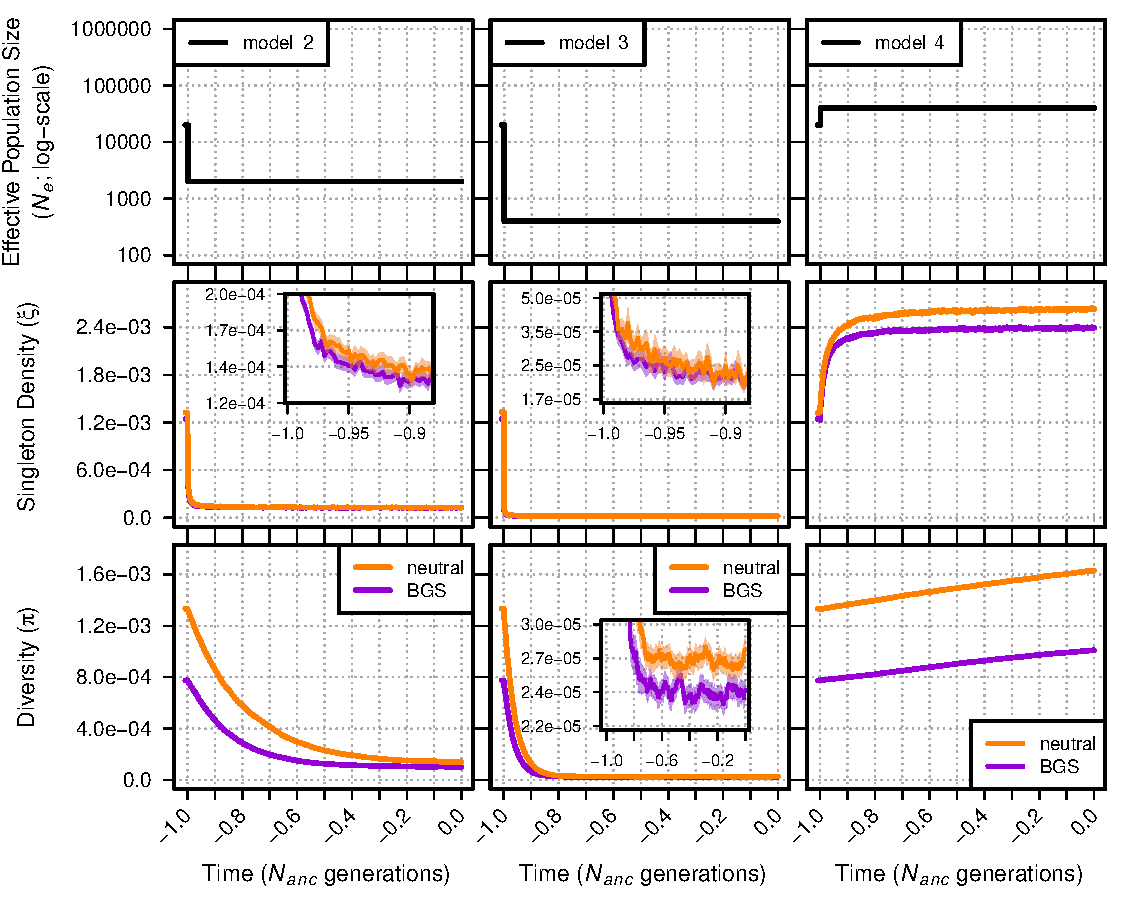
\includegraphics[width=\linewidth]{figures/FigS6.pdf}
\caption{Singleton density ($\xi$ per site) and diversity ($\pi$ per site) for models 2-4.
The top panel shows each demographic model; time proceeds forward from left to right and is scaled by the $N_e$ of the population at the initial generation ($N_{anc}$).
Diverstiy statistics are shown for neutral simulations (orange lines) and simulations with BGS (violet lines).
Insets show diversity using a log scale for improved detail.
Envelopes are 95\% CIs calculated from 10,000 bootstraps of the original simulation data.}
\label{fig:S6}
\end{figure}

To examine the interaction of demography and selection observed in empirical data \citep{beissinger2016recent,torres2018human}, we normalize $\pi$ and $\xi$ in models of BGS by their equivalent statistics generated under the same demographic model in the absence of any selection ($\pi_0$ and $\xi_0$).
We observed that $\pi/\pi_0$ and $\xi/\xi_0$ were dynamic through time in response to demography, with changes occurring to both their magnitude and direction (Figure \ref{fig:1}). 
Moreover, changes to $\xi/\xi_0$ occurred more rapidly through time when compared to $\pi/\pi_0$.
For example, in model 2 we observed a dip and rise in the $\xi/\xi_0$ statistic relative to the equilibrium model 1 within the first $\approx 0.1N_{anc}$ generations ($N_{anc}$ refers to the $N_e$ of the ancestral population prior to any demographic change).
Yet, for the same model, $\pi/\pi_0$ remained depressed for over $0.5N_{anc}$ generations (Figure \ref{fig:1}).
Similar patterns were observed for model 3, which experienced a greater reduction in size, although the pattern is less clear due to the greater sampling variance of $\xi/\xi_0$ due to the overall lower number of singletons.
In both models, both $\pi/\pi_0$ and $\xi/\xi_0$ appeared to plateau at levels above that of model the equilibrium model 1.
Under a model of simple population expansion (model 4) we observed markedly different dynamics, with a sustained increase in $\pi/\pi_0$ but only a transient increase in $\xi/\xi_0$ within the first $\approx 0.1N_{anc}$, followed by a reduction to levels below that of the equilibrium model.

\begin{figure}[]
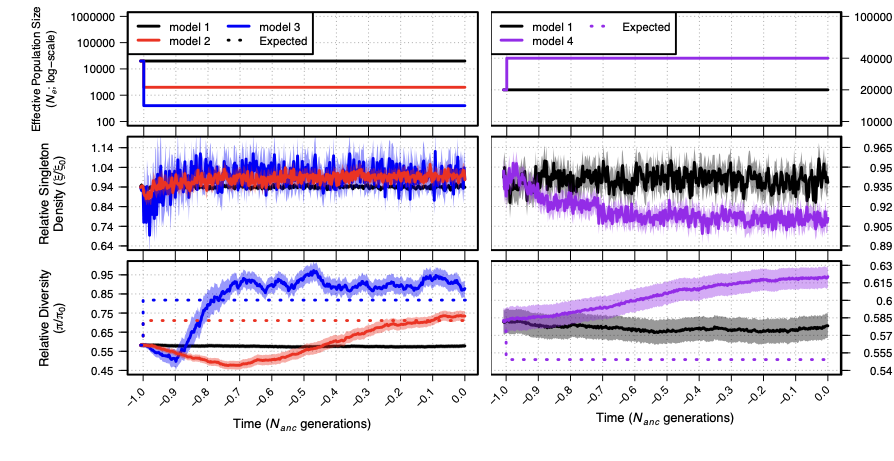
\includegraphics[width=\linewidth]{figures/tempF1.png}
\caption{Relative singleton density ($\xi/\xi_0$) and relative diversity ($\pi/\pi_0$) across time for demographic models 1-4.
The top panel shows each demographic model as in Figure \ref{fig:1}.
Black lines show $\xi/\xi_0$ and $\pi/\pi_0$ from simulations of a constant sized population (model 1).
Dotted lines in the bottom panel show the instantaneous expectation of $\pi/\pi_0$ from  \citet{nordborg1996effect} given the specific selection parameters and the instantaneous $N_e$ at each time point.
Envelopes are 95\% CIs calculated from 10,000 bootstraps of the original simulation data.}
\label{fig:1}
\end{figure}

Changes in population size should lead to changes in the rate of genetic drift and the efficacy of natural selection and, thus, changes in the magnitude of BGS across time.
Indeed, under equilibrium contions, the classic model of BGS \citep{nordborg1996effect} predicts weaker BGS (with higher $\pi/\pi_0$) for smaller populations and stronger BGS (with lower $\pi/\pi_0$) for larger populations.
To compare these prediction to those of our simple demographic models, we calculated the predicted $\pi/\pi_0$ under the classic mdoel given the instantaneous $N_e$ at each time point.
In all three simple demographic models, however, we observed that changes in $\pi/\pi_0$ over the short term were qualitatively opposite of predictions from the classic model  (Figure \ref{fig:1}; bottom panel).
The classic model predicts a higher value for $\pi/\pi_0$ in a smaller population, yet we observed a transient drop in $\pi/\pi_0$ directly after a bottleneck (models 2 and 3).
Similarly, while the classic model predicts a decrease in $\pi/\pi_0$ in larger populations, we observed a sustained increase in $\pi/\pi_0$ with population expansion (model 4) extending over the entire $N_{anc}$ generations of the simulation.
% Even though $\xi/\xi_0$ and $\pi/\pi_0$ experienced
% drops immediately in response to the population reductions of models 2
% and 3, these patterns of reduced $\xi/\xi_0$ and
% $\pi/\pi_0$ reversed themselves through time and, in the case
% of $\pi/\pi_0$, approached the expectation predicted by the
% Nordborg model.


\subsection{Babckground selection under bottleneck-expansion models}

We built upon the simple two epoch demographic scenarios to test more
complex demographic scenarios and their effects on patterns of diversity
under BGS. Specifically, we incorporated a bottleneck-expansion model
where we simulated a population undergoing a contraction similar in size
to models 2 and 3, but with a subsequent expansion to 400,000
individuals by the final generation. Although we vary the time length of
the contraction and expansion events (see Table 1), these
bottleneck-expansion models qualitatively match the demography of
previous empirical studies investigating the impact of BGS in dynamic
populations [20,51]. They also helped to glean information about
which particular demographic events --- contractions or expansions --- dominate the overall patterns that we witnessed for the two epoch models described previously.

For the demographic models in which the bottleneck event began -1.0
$N_{anc}$ generations in the past and was followed by
immediate expansion (models 5-6), we observed transient decreases in
$\xi/\xi_0$ and $\pi/\pi_0$, recapitulating the
dynamics observed for models 2 and 3 (Figure 3). Similar to models 2 and
3, we also observed approaches to higher values of $\pi/\pi_0$
later in their demographic histories, consistent with the effects of
weakened BGS as a result of the initial population decline. This was in
contrast to the decreasing $\pi/\pi_0$ expected for an
expanding, larger population (Figure 3; dotted lines). The approach to
higher $\pi/\pi_0$ values later in the demographic model also
occurred more rapidly for model 6 than model 5. Thus, as was shown when
comparing model 3 to model 2, the time to equilibrium after a size
change is highly dependent on $N_e$ and occurs more
quickly for populations suffering larger reductions. The fact that these
patterns of increasing $\pi/\pi_0$ exist despite the population
expansion events of models 5 and 6 also demonstrates the dominant
effects that a population decline has on patterns of diversity under
selection at linked sites.

While the population expansion eventually did have an effect on
increasing $\pi$ under both BGS and neutrality after the initial reduction
in size, this increase occurred at a higher relative rate under BGS and
was further accelerated by larger reductions in population size. This is
evident in Figure S7 where we compared $\pi$ relative to its initial value
through time. There, we observed a sharper increase in $\pi$ under BGS
following its minimum point for model 6 when compared to model 5.
However, for both models, the faster rate of recovery of $\pi$ under BGS in
response to the expansion also ensured that $\pi/\pi_0$
continued to remain higher in later generations. So while bottlenecks
led to a sharper rate of decrease in $\pi$ under BGS when compared to
neutrality, they also aided in a faster rate of recovery during the
expansion, thereby leading to an increase in $\pi/\pi_0$ in the
face of growth and mimicking patterns evident for models with no
expansion. The fact that the approach to higher $\pi/\pi_0$
occurred \emph{despite} the increasing population size of both
demographic models clearly demonstrated that patterns of
$\pi/\pi_0$ were primarily being driven in response to earlier
demographic events (i.e., the initial population contraction). Yet the
stronger action of BGS in response to population expansion should
eventually arise for both models and is suggested by the decreasing $\pi$/$\pi_0$ predicted by the Nordborg model (Figure 3; dotted
lines). Such patterns may take much longer to manifest than the time
span we have simulated here if approaches to equilibrium take on the
order of $4N_e$ generations [28,58].

Observations of the dominant impact of genetic drift and weakened BGS
following a population reduction were also apparent when measuring
patterns of $\pi/\pi_0$ in models that had a more sustained
contraction (i.e., models 7 and 8). There, a decline in
$N_e$ was sustained for an additional 0.5
$N_{anc}$ generations before the expansion event began
(Figure S2). For these models, the rise of $\pi/\pi_0$
resulting from weakened BGS occurred more quickly than for their
counterpart models with an immediate expansion (Figure S3). For example,
the inflection point at which $\pi$ under BGS surpassed $\pi$ under neutrality
occurred at -0.305 and -0.848 $N_{anc}$ generations
for models 7 and 8, respectively (Figure S7). For models 5 and 6, these
inflection points occurred later in time at -0.235 and -0.785
$N_{anc}$ generations, respectively. Further, the
final $\pi/\pi_0$ values for models 7 and 8 were 0.643 and
0.887 but for models 5 and 6, they were only 0.631 and 0.860. Thus, the
sustained lower $N_e$ of models 7 and 8 aided in
accelerating the approach to the new equilibrium established by
population reduction. This provided further evidence for the dominant
role that population bottlenecks have for patterns of diversity under
BGS, even when populations expand past their ancestral size.

It is possible that the expansion itself has contributed to the rise in
$\pi/\pi_0$ for models 5-8, as was seen for model 4. However,
this is unlikely to be the case because the rise in $\pi/\pi_0$
occurred fastest for models 7 and 8, which had a delayed onset of
expansion. Second, this rise occurred faster still for models 2 and 3,
which had no expansion in size. There, the inflection point at which $\pi$
under BGS surpassed $\pi$ under neutrality occurred at -0.44 and -0.865
$N_{anc}$ generations for models 2 and 3, respectively
(Figure S9). Rather, the population expansion of models 5-8 appeared to
retard the approach to equilibrium in response to their size reductions,
thus preventing $\pi/\pi_0$ from attaining higher values. When
comparing each respective model's maximum $\pi/\pi_0$, we
observed that models 2 and 3 both had the highest values given their
respective population reductions to 2,000 and 400 individuals
($\pi/\pi_0$ = 0.738 and 0.972, respectively; Figure 1). This
was followed by models 7 and 8 ($\pi/\pi_0$ = 0.644 and 0.887,
respectively) and finally, by models 5 and 6 ($\pi/\pi_0$ =
0.631 and 0.861, respectively; Figure 3). Thus, those models
experiencing the shortest amount of time at reduced population sizes saw
the lowest rises in $\pi/\pi_0$. For models 5-8, though,
$\pi/\pi_0$ was still approaching higher values since these
models were not at equilibrium after 1.0 $N_{anc}$
generations. It is likely that $\pi/\pi_0$ for these models
would attain even higher values if their demographic histories were
extended.

In contrast to $\pi$, the loss and gain of $\xi$ and change to
$\xi/\xi_0$ in response to the bottleneck-expansion models was
much more rapid and dynamic through time. This was expected since rare
variants (e.g., singletons) are more likely to be lost during a
contraction, and during an expansion injection of new mutations fill
these bins in the SFS first. For models 5 and 6, we witnessed a very
brief dip in $\xi/\xi_0$, resulting from a greater relative
decrease in $\xi$ under BGS when compared to neutrality (Figure 3; Figure
S7). Following this dip, $\xi$ under BGS increased at a relatively faster
rate than $\xi$ under neutrality, resulting in a higher $\xi/\xi_0$
relative to their initial values (Figure S7). Similar patterns were also
seen for models 7 and 8 (Figure S3, Figure S7). Qualitatively, these
first directional changes in $\xi/\xi_0$ matched those of
$\pi/\pi_0$, but occurred over a much shorter time span. These
changes were likely a consequence of regime change from the dominance of
genetic drift immediately following the population reduction to the
dominance of weakened BGS from a reduced $N_e$. This
was previously exhibited by models 2 and 3 and additional evidence for
this was provided by the observation that changes in the magnitude of
$\xi/\xi_0$ were greater for model 6 and model 8 than for model
5 and model 7 (i.e., greater for models suffering larger reductions in
$N_e$).

Because the dynamics of rare variants are more sensitive to demography,
we also witnessed another change in the direction of
$\xi/\xi_0$ that was not observed for $\pi/\pi_0$.
Following an increase in $\xi/\xi_0$ above its initial point
from weakened BGS, we saw a decrease later in time, with
$\xi/\xi_0$ falling below that initial point by -0.2
$N_{anc}$ generations (Figure 3, Figure S3). This last
decrease in $\xi/\xi_0$ could not have resulted from an
increased sensitivity to drift because the population sizes were larger
during this phase of the demography (79,636 $N_e$
and 57,722 $N_e$ at -0.2 $N_{anc}$
generations for models 5 and 6, respectively). Rather, BGS appeared to
act more strongly in these later generations and, thus, limited $\xi$
relative to its value under neutrality. Supporting this, we observed a
slower rate of increase in $\xi$ under BGS towards the very end of the
expansion for models 5-8 (Figure S4; Figure S7). Finally, we observed
that the final $\xi/\xi_0$ value for model 5 was lower than for
model 6 (0.881 vs. 0.893) and the final $\xi/\xi_0$ value for
model 7 was lower than for model 8 (0.879 vs. 0.896) (Figure S3). This
may have resulted from the fact that models 5 and 7 had higher long term
$N_e$ and experienced a concomitantly stronger
amount of BGS throughout their history due to their shallower population
bottlenecks.

We also ran a set of simulations with demographic histories simulating
the effects of more recent bottlenecks on patterns of
$\pi/\pi_0$ and $\xi/\xi_0$ (models 9-12; Figure S2).
These models were similar to models 5-8, with identical starting and
ending population sizes and population size reductions. For these
models, we observed similar patterns in response to the population
reductions seen in the previous models. In all cases,
$\pi/\pi_0$ suffered a decrease, which was once again in
contrast to the expectation given by the Nordborg model (Figure S3).
Also similar to the previous models, $\xi/\xi_0$ for models
9-12 suffered a transient decrease followed by a recovery over its initial value.
For models 9 and 10, which both had an immediate
expansion following their size reductions, the magnitude of loss for $\pi$
and $\xi$ was less than for their counterpart models -- models 5 and 6
(compare Figure S4 to Figure S5). This result likely stemmed from the
higher rate of population growth necessary to end at a size of 200,000
individuals over the course of 0.1 $N_{anc}$
generations for models 9 and 10, which mitigated the greater loss of $\pi$
and $\xi$ exhibited by models 5 and 6. Additionally, the decrease in
$\pi/\pi_0$ was less for models 9 and 10 when compared to
models 5 and 6. After 0.1 $N_{anc}$ generations,
$\pi/\pi_0$ was 0.545 and 0.492 for models 5 and 6,
respectively but 0.573 and 0.541 for models 9 and 10, respectively
(Figure S3). This demonstrated the effects of the greater rate of
expansion on limiting the sensitivity to drift in regions of BGS.
Further, for models 11 and 12, which had a delayed expansion, measures
of $\pi/\pi_0$ were also lower than for models 9 and 10 after
$0.1N_{anc}$ generations, exhibiting values of 0.542
and 0.527, respectively (Figure S3). These models also clearly
demonstrated the feature of $\xi$ under BGS not only declining more quickly
in magnitude immediately following the population contraction but also
recovering more quickly once it reached its minimum, thus displaying the
more rapid behavior characteristic of patterns of diversity under the
effects of BGS and demography. Specifically, when comparing $\xi$ under BGS
to $\xi$ under neutrality, $\xi$ under BGS in the final generation was
relatively higher than its initial value (Figure S8). This caused the
elevated $\xi/\xi_0$ exhibited in the final generation of
models 9-12 (Figure S3).

Because the history of models 9-12 only lasted 0.1
$N_{anc}$ generations, we also observed much more
limited dynamics of $\pi/\pi_0$ and $\xi/\xi_0$.
Specifically, $\pi/\pi_0$ did not recover above its initial
starting point by the final generation and $\xi/\xi_0$ did not
decrease in response to the population expansion, but rather continued
to remain elevated (Figure S3). These features are important because
they demonstrated that qualitatively similar demographic events, such as
the bottleneck-expansion model shared by models 5-8 and 9-12, can yield
opposite trends in statistics used as proxies for measuring the
intensity of BGS. Thus, the resulting effects on patterns of relative
diversity under BGS depend on how far removed the point of observation
is from a particular demographic event. Such patterns also help to
reconcile the qualitatively different observations yielded by previous
studies [20,51] (discussed further below).

\subsection{Patterns of $\pi/\pi_0$ and $\xi/\xi_0$ across
200 kb neutral region}

We also measured patterns of $\pi/\pi_0$ across time for the
entire 200 kb neutral region. Doing so showed the characteristic
``trough'' structure of increasing relative diversity as a function of
genetic distance from the focl locus under selection (Figure 4, Figures
S10-S20). For the two-epoch models with a population contraction (models
2-3) we observed that the slope of the trough became more shallow
through time, with the difference between the closest 10 kb bin and
farthest 10 kb bin from the 2 Mb selected locus decreasing between the
initial and final generations (Figures S10-S11, Table 4). Thus, the
impact of population contractions on mitigating the effects of BGS
resulted in larger shifts of $\pi/\pi_0$ in regions of the
genome already under the strongest amount of BGS. This makes sense since
regions farther removed from loci under purifying selection (i.e., under
weaker effects of BGS) have values of $\pi/\pi_0$ closer to the
neutral expectation of 1. Thus, the upper bound for change in
$\pi/\pi_0$ will be more limited there compared to regions more
proximal to a selected locus. However, the decrease in the slope of the
trough was initially minimal and only accelerated after
$\pi/\pi_0$ across the 200 kb region reached its minimum values
(Table 4). This provided further evidence for the dominant effects of
drift and allelic loss on driving the initial decrease in
$\pi/\pi_0$ immediately following a population contraction,
which should have unbiased effects across all bins within the trough.
During the subsequent recovery to higher values of $\pi/\pi_0$, we saw smaller differences arise
between the nearest and farthest 10 kb bins, demonstrating the expected
weakening effects of BGS following a population decline. This weakening
of the trough structure was also most apparent for model 3, with
patterns of $\pi/\pi_0$ appearing essentially flat across the
200 kb region in the final generation (Figure S11).

We observed similar patterns for the bottleneck-expansion models that
lasted 1 $N_{anc}$ generations (Figures S13-S16).
Notably, among those models, the slope of the trough became more shallow
for models 6 and 8 which were also the models suffering the deepest
reductions in size (Figures S14, S16; Table 4). The fact that the trough
structure for models 5 and 7 was better maintained showed that the
population expansion following the reduction in size kept BGS stronger
through time relative to models with the same decline in size but
without a recovery (e.g., model 2). Models lasting 0.1
$N_{anc}$ only captured the decrease of
$\pi/\pi_0$ due to drift and saw very little difference develop
across their troughs (Figures S17-S20). Similarly, for model 4, the
trough structure remained unchanged throughout its demographic history
(Figure S12).

Finally, repeating the same analysis across the 200 kb regions for
$\xi/\xi_0$ yielded no discernible patterns. Troughs were
slightly apparent for the final generations of some models (i.e., models
5 and 7), but the stochasticity between windows for $\xi/\xi_0$
swamped any obvious patterns across the 200 kb region through time.
Since $\xi/\xi_0$ is already less affected (and, thus, closer
to 1) than $\pi/\pi_0$ because BGS perturbs common frequency
bins of the SFS more than rare ones [57], any signal using rare
frequency bins will be inherently more difficult to capture across
differing magnitudes of BGS. However, more extensive simulations may
help to uncover such patterns.


%%%%%%%%%%%%%%%%%%%%%%%%%%%%%%%%%%%%%%%%%%%%%%%%%%%%%%
\section{Discussion}
%%%%%%%%%%%%%%%%%%%%%%%%%%%%%%%%%%%%%%%%%%%%%%%%%%%%%%

%behavior of $\pi/\pi_0$ and $\xi/\xi_0$ in simple demographic models
%models2-3
While the effects of BGS should be attenuated in populations with lower $N_e$ (because the efficacy of purifying selection is weakened), the drop in $\pi/\pi_0$ instead demonstrated that the populations were dominated by the effects of allelic loss, which is expected for populations suffering a strong bottleneck.
Additionally, more rapid effects were observed for model 3s despite the fact that the expectation of $\pi/\pi_0$ for model 3 was actually higher than for model 2.
These observations made it clear that effects of BGS on $\pi/\pi_0$ immediately following a reduction in $N_e$ were not driven by a change in the efficacy of natural selection from population decline, but rather by the increased sensitivity of allelic loss within these regions -- with greater rates of loss accompanying greater reductions in population size.
The diversity-reducing effects of BGS have often been modeled as a reduction in $N_e$ [56], which has been observed to increase sensitivity to drift for populations experiencing recent bottlenecks [51] (though we caution that effects of BGS on the SFS cannot be simplified to this extent [57]).
These patterns were made evident when observing the more rapid relative decrease in diversity in our selection models with BGS versus neutrality.
% When compared to their initial equilibrium starting points, $\pi$ under BGS suffered faster rates of loss compared to the neutral case for both models (Figure S9), with the fastest rates of loss accompanying larger reductions in $N_e$ (i.e., model 3).
Importantly, these results demonstrated that classical models that predict the impact of BGS on $\pi/\pi_0$, such as the Nordborg model, implicitly assume an equilibrium population at  mutation-selection balance [58] and are inappropriate for predicting true patterns of genetic diversity for populations that have udnergone recent size changes.

 These dynamics occurred more quickly for
$\xi/\xi_0$, which was expected since approaches to equilibrium
are more rapid for rare variants relative to common variants.
Additionally, the approaches to equilibrium occurred fastest for model
3, which also suffered the larger population size reduction (Figure 1).
This faster approach was also not unexpected since, in general, the time
to equilibrium is scaled by $N_e$ [28,58] and
changes resulting in smaller $N_e$ (e.g., model 3)
should also result in shorter times towards new population equilibria.
Thus, despite the demographic change resulting in immediate decreases to
$\xi/\xi_0$ and $\pi/\pi_0$, patterns of relative
diversity in populations suffering a contraction eventually approached
their expected higher equilibrium values under weakened BGS, with rates
dependent on the frequency of the alleles being observed and the
magnitude of the population reduction. This was evident from the fact
that the final $\pi/\pi_0$ values for models 2 and 3 were
within close approximation of the Nordborg model. However, we note that
this expectation underestimated $\pi/\pi_0$ for model 3 because
the threshold of $s < 0.15/2N_e$
was likely not conservative enough to ignore deleterious mutations that
behave neutrally under the low $N_e$ size of 400 for
that model.


%model4
The latter pattern occurred despite the
expectation of a decrease in $\pi/\pi_0$ from the Nordborg
model, which would have been generated by more efficient purifying
selection accompanying a larger $N_e$.

The more sensitive and rapid response to population increase under BGS
recapitulated the faster approaches to equilibrium that were exhibited
in the contraction models. Intuitively, these faster approaches to new
equilibrium levels under BGS in response to size changes make sense if
we consider the fact that the distance between initial and final
equilibrium diversity levels for both $\pi$ and $\xi$ are closer to one another
under BGS when compared to neutrality (Figure S6; Table 2-3). This
provided a potential explanation for why we observed the specific
dynamics of $\pi/\pi_0$ immediately following a size change.
This argument likely does not hold for model 4 because, due to its
higher $N_e$, it is unlikely that equilibrium has
yet been reached. However, the observation of an increase in
$\pi/\pi_0$ for model 4 did provide supporting evidence that a
faster approach to equilibrium under BGS still existed under an
expansion model. Indeed, moderl 4 $\pi$ under BGS changed more quickly than
under neutrality (Figure S9). Presumably, this also indicates that $\pi$
under BGS will reach a new equilibrium first, at which point
$\pi/\pi_0$ will begin a downward trajectory in response to $\pi$
continuing to increase under neutrality but $\pi$ under BGS remaining at a
constant equilibrium. This is a likely outcome if the qualitative
changes in $\xi/\xi_0$ foreshadow the future dynamics of
$\pi/\pi_0$. The end result would also include a decrease in
$\pi/\pi_0$ relative to its initial starting point, with
$\pi/\pi_0$ eventually reaching a value close to its
expectation (Figure 2; dotted lines). Although we foresee no reason why
this prediction should not hold true, more extensive simulations will be
necessary to confirm this.

%%%%%%%%%%%%%%%%%%%%%%%%%%%%%%%%%%%%%%%%%%%%%%%%%%%%%%
\section{Conclusion}
%%%%%%%%%%%%%%%%%%%%%%%%%%%%%%%%%%%%%%%%%%%%%%%%%%%%%%

Recently, two empirical investigations into the joint impacts of
demography and selection at linked sites in the context of BGS yielded
interesting and intuitive, albeit contradictory, observations.
Beissinger et al. [20] conducted a study across 36 samples from
maize and its wild progenitor teosinte. They found that patterns of
relative genetic diversity (i.e., $\pi/\pi_0$) across regions
experiencing linked selection in maize, which underwent a demographic
bottleneck during domesticaiton, were higher than in teosinte. They
attributed this to the historically larger $N_e$ of
teosinte, which led to more efficient natural selection and thus a
greater impact of BGS on neutral diversity. However, the contemporary
population size of maize, a staple food crop grown world-wide, is now
much larger than teosinte and should be experiencing stronger selection
in its recent history. Supporting this hypothesis, relative singleton
density of neutral sites in maize, which should reveal more recent
signals of evolutionary history, was lower compared to teosinte.
However, Torres et al. 2018 [51] revealed opposite patterns in
humans. There, through a analysis of over 2,500 human genomes, they
observed that relative genetic diversity ($\pi/\pi_0$) was
lower in non-Africans, a population that has undergone a series of
extensive population bottlenecks and exhibits a low long-term
$N_e$, when compared to Africans. Additionally,
relative singleton density was also higher in non-Africans. In
conclusion, the authors attributed these patterns to a higher
sensitivity to demography and drift in regions of selection at linked
sites, thus yielding lower relative diversity in bottlenecked
populations. They also concluded that the greater long-term
$N_e$, and thus more effective purifying selection
and greater BGS, of Africans has led to their observed lower relative
singleton density.

While these patterns observed in maize and humans are seemingly in
disagreement, important demographic details, such as the length of the
population bottleneck and the time since the post-bottleneck population
expansion began, may also be significant contributors to these results.
As our simulations demonstrated, it is possible for two qualitatively
similar demographic histories to yield opposite patterns if the window
of time in which those patterns are observed are different. In the case
of maize compared to teosinte, observations are being made at a time in
which BGS is operating less effectively on removing average pairwise
diversity (due to its lower long-term $N_e$) but
more effectively on singletons (due to its higher contemporary
$N_e$). But if this population had been sampled more
closely to its population bottleneck event, observations of relative
diversity may have been more aligned with what is currently observed for
humans. The approximate number of generations removed from the
domestication bottleneck event for maize is about 15,000 generations
[20]. For humans, the approximate number of generations removed from
the out-of-Africa bottleneck event is only 6,000 generations [51].
Therefore, it is not unreasonable to suspect that these different
timespans contribute to the qualitatively different observations now
being observed.

Importantly, these two studies provide striking examples of the
importance of considering the impact of demography and time on extant
patterns of diversity to avoid mis-attributing the underlying forces
driving those patterns in regions experiencing selection at linked
sites. Since the null expectation of a natural population should be that
it is not at demographic equilibrium [59], alternative hypothesis
testing on selection at linked sites should also include the effects of
non-equilibrium demography and how they affect patterns though time.
However, in the specific context of maize and humans, we also note that
other details, such as the periodic bottlenecks suffered by non-Africans
(which may have further accelerated drift) and the differences among the
distribution of fitness effects for these two species, are equally
important to consider and warrant further investigation as well.

Recent model development incorporating demography into models of BGS
holds promise on generating demographically aware models on the effects
of selection at linked sites in populations. In particular, results from
Zeng 2013 [48], which formulated a simulation-based structured
coalescent model of BGS with demography, also showed that demography can
perturb levels of genetic diversity under BGS through time. In a
separate study, an analytical model which is capable of incorporating
changing demography was formulated and will prove more ideal for
performing inference of selection at linked sites in dynamic populations
[49]. Both of these models, though, are limited in their ability to
accurately predict the effects of selection at linked sites when
mutation-selection balance breaks down, which typically occurs when the
population scaled selection coefficient, $\gamma$, approaches 1. In
general, the deterministic approximation implicit for models of BGS may
not be suitable for $\gamma \leq 3$ [56]. During the course of a
bottleneck, as we have simulated here, $\gamma$ is likely to fall below
these thresholds and patterns of diversity may be more strongly affected
by other processes such as genetic drift or the ``interference
selection'' regime described in Good et al. 2014 [60]. For the case
in which $s$ is drawn from a skewed distribution, such as the gamma
distribution, the deterministic approximation is further likely to break
down when $s$ is small. We attempt to limit these specific issues
in the Nordborg model by simply truncating $s$ so that predictions
better match observed levels of BGS for various population sizes
(albeit, under the additional assumption of demographic equilibrium).
This simplistic approach may be suitable for other models of BGS, but as
our results showed, it will likely provide only a coarse estimate for
the prediction of diversity under BGS (Figure S21).

\hyperdef{}{ux5f30j0zll}{}{}Finally, our results extend the recent
debate on patterns of diversity in selected sites in non-equilibrium
populations (especially in humans [61--64]) to patterns of diversity
across neutral sites. For the specific case of selected sites, sites
under strong selection are more sensitive to demographic change and will
reach new equilibrium frequency levels more quickly than neutral sites
or weakly selected sites [65--67]. As we have shown here in the
context of neutral sites, because the underlying equilibrium frequency
of neutral sites depends on the strength of selection at linked sites,
demographic change will also result in distinct responses to their
change in frequency. In addition, the rate of change will also depend on
which bins of the SFS diversity is being measured with. Together, this
results in the complex change of $\pi/\pi_0$ and
$\xi/\xi_0$ through time that we observed from our simulations.
This insight should provide caution, however, for studies attempting to
uncover the action of natural selection by comparing sites within the
genome since, even when controlling for the strength of BGS itself,
frequencies of neutral sites may still be at different relative levels
depending on the recent demographic history of the population.

\section{Acknowledgments}


\bibliography{example-bibliography}

%\pagebreak
\onecolumn

\beginsupplement
\section*{Supplement}

\begin{figure*}[h!]
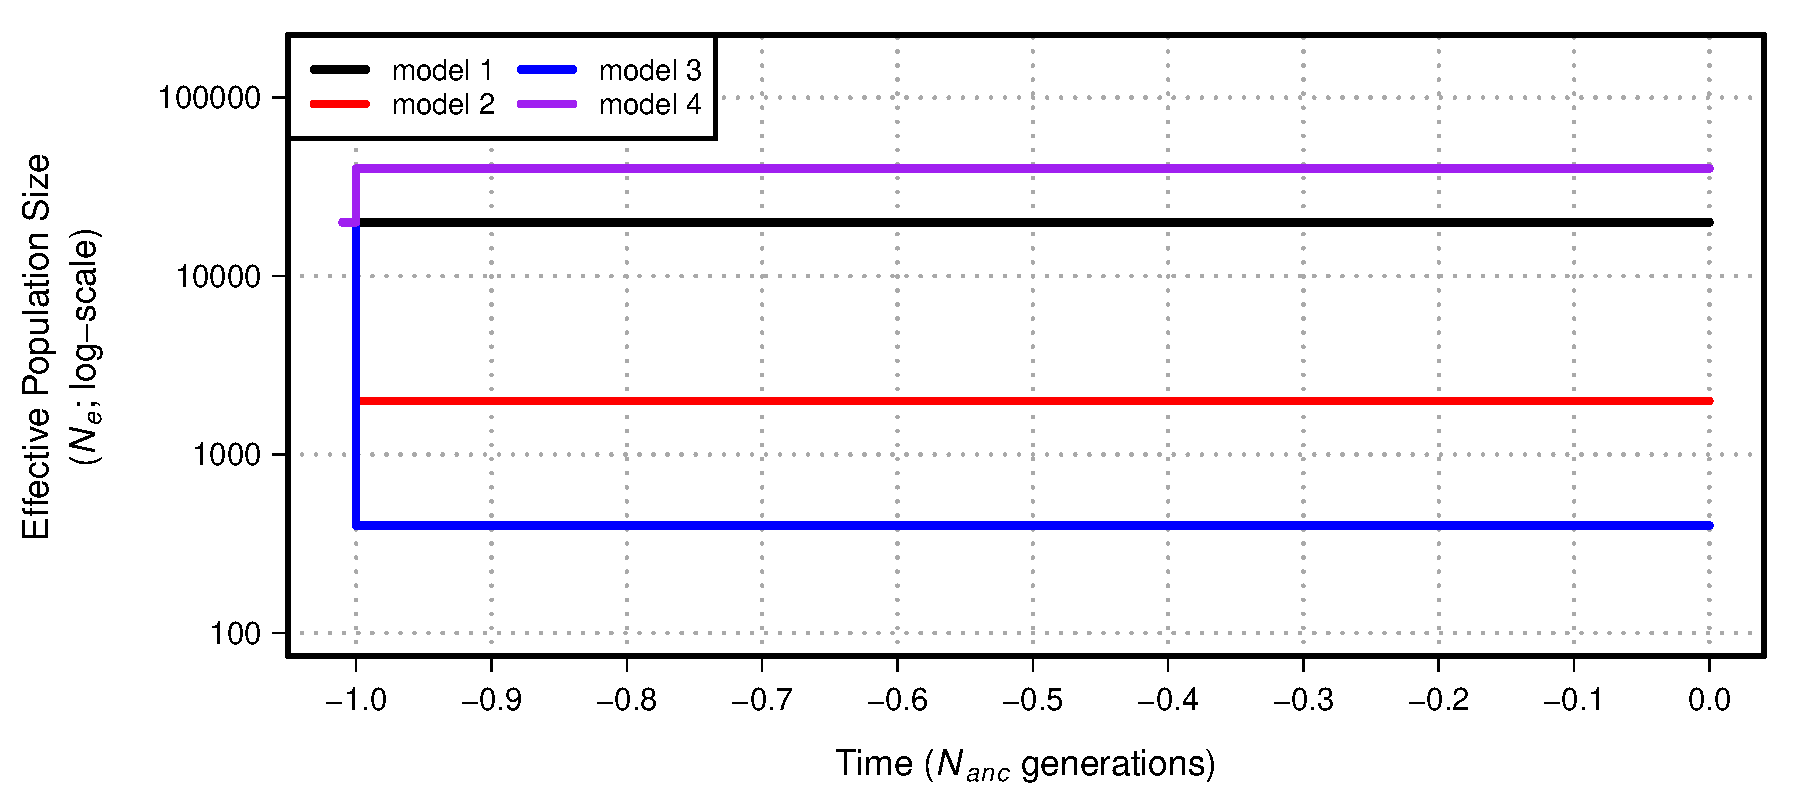
\includegraphics[width=0.8\linewidth]{figures/FigS1.pdf}
\caption{Demographic models 1-4 simulated in our study.
Time proceeds forward from left to right and is scaled by the $N_e$ of the population at the initial generation ($N_{anc}$; 20,000 individuals).
Demographic model 2 experiences a population contraction to 2000 individuals while demographic model 3 experiences a population contraction to 400 individuals.
Demographic model 4 experiences a population expansion to 40,000 individuals.
All population size changes are instantaneous for models 2-4.
See Table \ref{table:params} for additional model parameters.}
\label{fig:S1}
\end{figure*}
\pagebreak

\begin{figure*}[t]
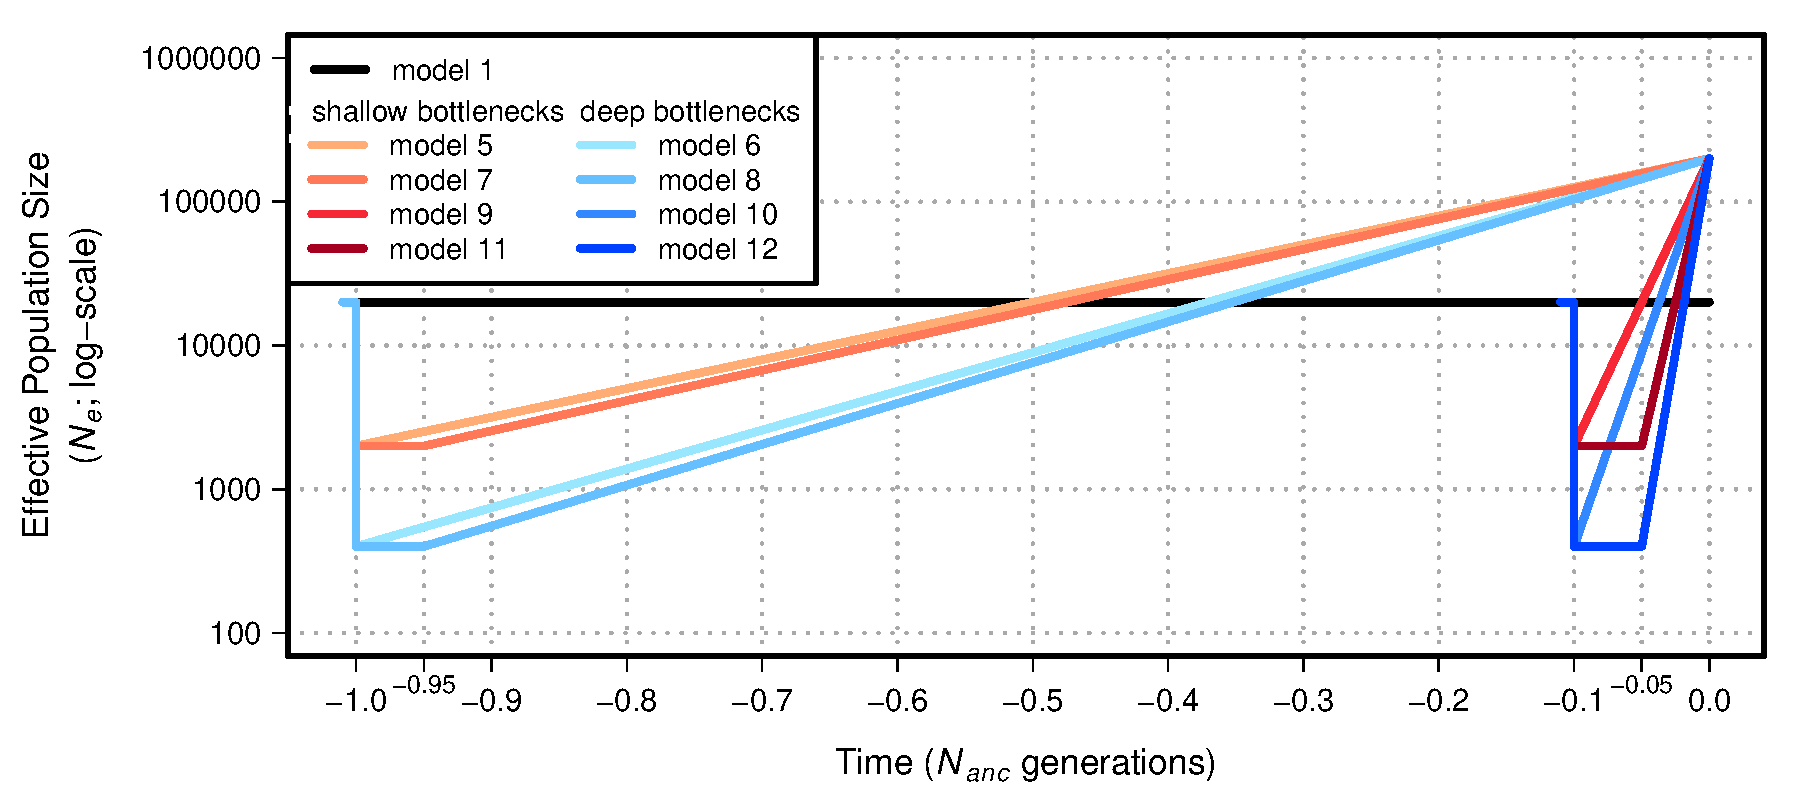
\includegraphics[width=0.8\linewidth]{figures/FigS2.pdf}
\caption{Demographic models 1 and 5-12 simulated in our study.
Time proceeds forward from left to right and is scaled by the $N_e$ of the population at the initial generation ($N_{anc}$; 20,000 individuals).
Demographic models experiencing a shallow bottleneck (models 5, 7, 9, and 11) experience a population contraction to 2000 individuals while demographic models experiencing a deep bottleneck (models 6, 8, 10, and 12) experience a population contraction to 400 individuals.
After contraction, demographic models 5-12 undergo exponential growth to a final population size of 200,000 individuals.
See Table \ref{table:params} for additional model parameters.}
\label{fig:S2}
\end{figure*}
\pagebreak

\begin{figure*}[t]
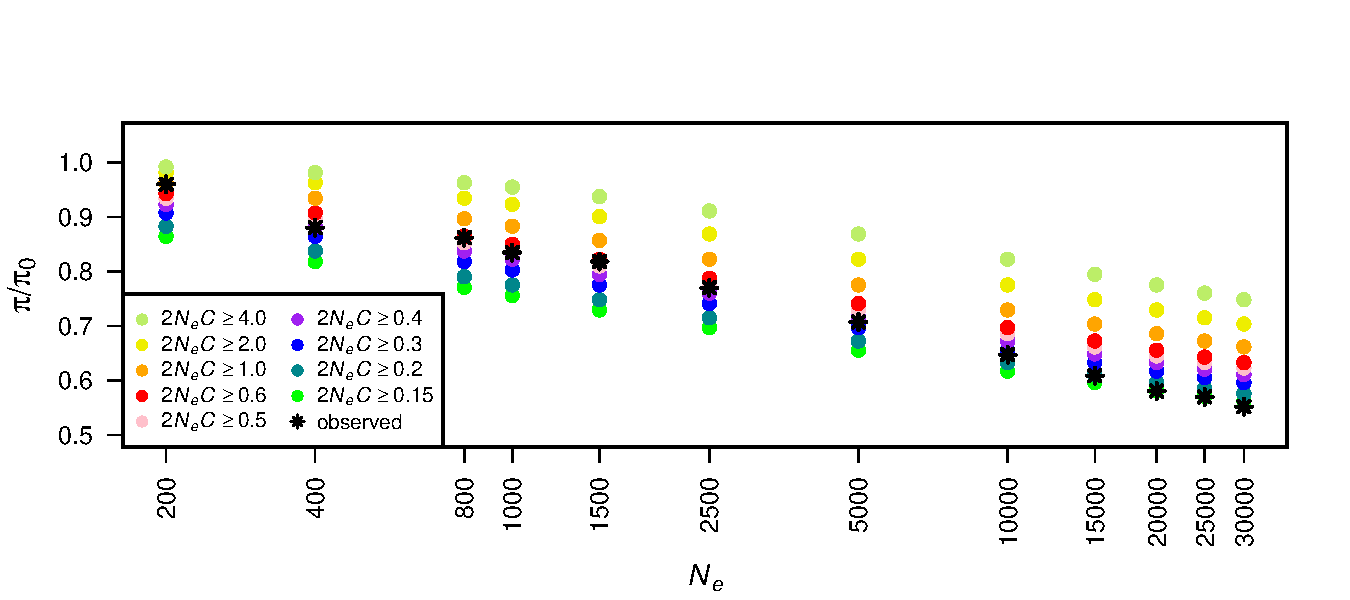
\includegraphics[width=.9\linewidth]{figures/FigS21.pdf}
\caption{Estimate of $\pi\pi_0$ from the Nordborg model across different population sizes and different truncation thresholds on selection.
Different $\gamma$ values used to truncate $s$ for the Nordborg model are shown in the legend ($2N_es \geq \gamma$).
Black stars represent the observed $\pi\pi_0$ from running simulations of BGS.}
\label{fig:nordborgsims}
\end{figure*}
\pagebreak

\begin{figure*}[t]
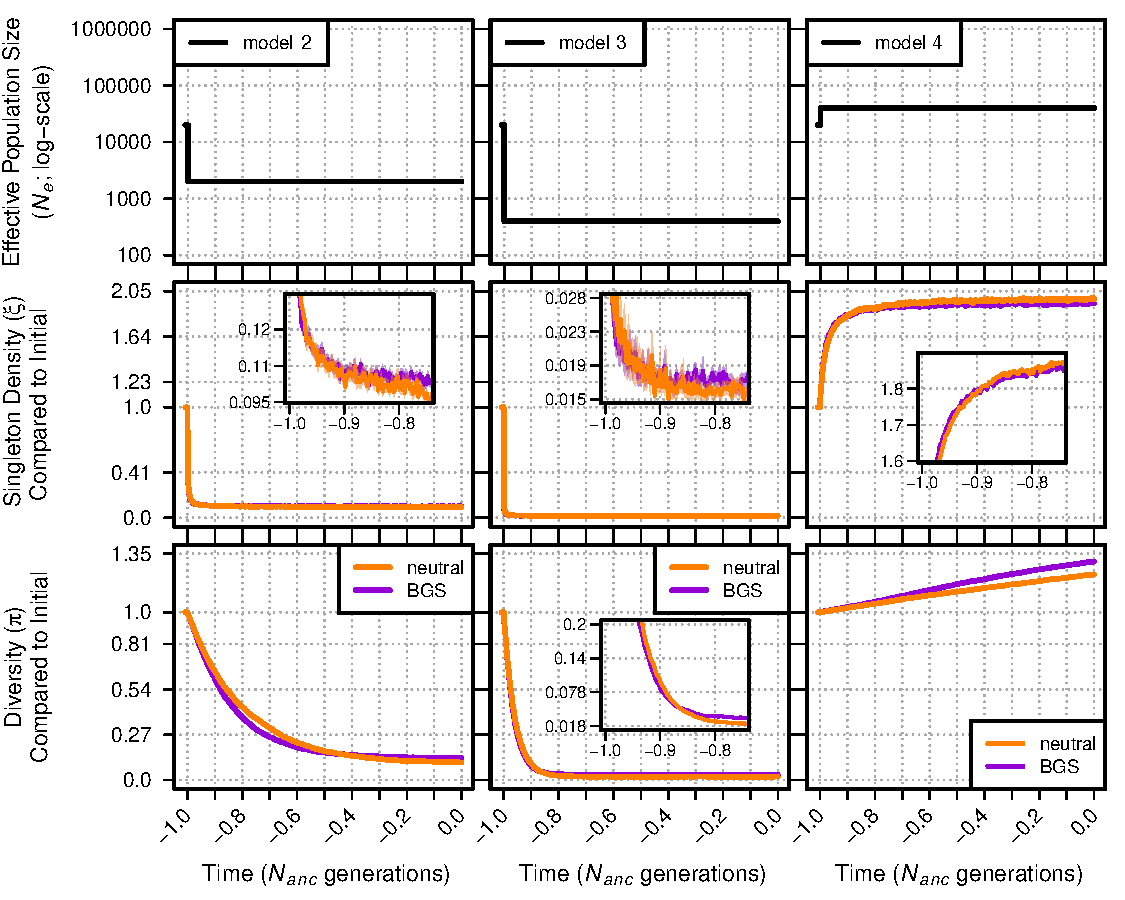
\includegraphics[width=.9\linewidth]{figures/FigS9.pdf}
\caption{Singleton density ($\xi$) and diversity ($\pi$) for demographic models 2-4 under neutrality (orange lines) and BGS (violet lines) relative to their values in the initial generation prior to demographic change.
The top panel shows each demographic model as in Figure \ref{fig:1}.
For greater detail, insets show data for generations over a smaller time scale and smaller y-axis (note: y-axes for insets are scaled linearly).
Envelopes are 95\% CIs calculated from 10,000 bootstraps of the original simulation data.
The data used for this figure is identical to that of Figure \ref{fig:1}.}
\label{fig:S9}
\end{figure*}
\pagebreak


% \begin{table*}[htbp]
% \centering

% \caption{\bf Shrink a large table to fit the page}
% %\begin{adjustbox}{totalheight=\textheight-2\baselineskip}
% \begin{tableminipage}{\textwidth}
% \begin{small}
% \begin{tabularx}{\textwidth}{sb}
% \hline
% Parameter & Description \\
% \hline
% \textbf{Adaptation} & \textbf{Trait related parameters} \\
% \hline
% Time to optimum & Generations until new optimum is reached \\
% Adaptation rate (haldane) & Adaptation rate until new optimum is reached. Calculated as $rate(h) = \frac{\frac{ln(x_2)}{sd_{x_{12}}}-\frac{ln(x_1)}{sd_{x_{12}}}}{t_2-t_1}$ \\
% Final genetic variance & Genetic variance in the final generation \\
% \textbf{Fixations} & \textbf{Mutations that fix after the optimum shift} \\
% \hline
% From new mutations (\#) & Sum of fixed mutations in the final population that were already segregating before  the optimum shift \\
% From standing variation (\#) & Sum of fixed mutations in the final population that arose after the optimum shift \\
% Max. effect size & Maximal effect size of all fixations \\
% Mean effect size & Mean effect size of all fixations \\
% Mean effect size of negative fixations & Mean effect size of negative mutations \\
% Mean effect size of positive fixations & Mean effect size of positive mutations \\
% Mean emergence time & Mean generation when a mutation arose that fixed in the last 0.1 N generations \\
% Mean fixation time & Mean generation in which a mutation fixed \\
% Min. effect size & Minimal effect size of all fixations \\
% Negative (\#) & Sum of fixed mutations with negative effects in the final population \\
% New/standing fixations & Ratio of mutations from new mutations vs. standing mutations  \\
% Proportion negative & Proportion of negative fixations from all mutations \\
% Positive (\#) & Sum of fixed mutations with positive effects in the final population \\
% SD of effect sizes & Standard deviation of effect sizes of all fixations \\
% SD of negative effect sizes & Standard deviation of effect sizes of negative fixations \\
% SD of positive effect sizes & Standard deviation of effect sizes of positive fixations \\
% Total (\#) & Sum of fixed mutations in the final population \\
% \textbf{Sweeps} & \textbf{Mutations that fix faster than 99\% of neutral fixations} \\
% \hline
% Hard sweeps (\#) & Sum of selective sweeps from new mutations \\
% Proportion of hard sweeps & Porportion of hard selective sweeps of all selective sweeps \\
% Proportion of sweeps from standing & Proportion of selective sweeps from stainding variation of all selection sweeps \\
% Sweeps (\#) & Sum of selective sweeps \\
% Sweeps from standing variation (\#) & Sum of selective sweeps from mutations that were already segregating before  the optimum shift \\
% Sweeps/fixations & Ratio of sweeps vs. fixations \\
% \textbf{Segregating sites} & \textbf{Mutations that segregate in the final generation} \\
% \hline
% Max. effect size & Maximal effect size of segregating sites \\
% Mean effect size & Mean effect size of segregating sites \\
% Mean effect size of negative sites & Mean effect size of segregating sites with negative effects \\
% Mean effect size of positive sites & Mean effect size of segregating sites with positive effects \\
% Mean frequency of all sites & Mean allele frequency of segregating sites \\
% Mean frequency of negative sites & Mean allele frequency of segregating sites with negative effects \\
% Mean frequency of positive sites & Mean allele frequency of segregating sites with positive effects \\
% Min. effect size & Minimal effect size of segregating sites \\
% Negative (\#) & Sum of segregating sites with negative effect \\
% Positive (\#) & Sum of segregating sites with positive effect \\
% Proportion of negative sites & Proportion of segregating sites with negative effect of all segregating sites \\
% Standard deviation of effect sizes & Standard deviation of effect sizes of all segregating sites \\
% Total (\#) & Sum segregating sites in the final generation \\
% \hline

% \end{tabularx}
%   \label{tab:parameter_list}
%   \end{small}
% \end{tableminipage}

% %\end{adjustbox}
% \end{table*}


\end{document}
